\section{La actualización dinámica de controladores como un problema de síntesis de controladores}

Una primera aproximación intuitiva para implementar la actualización de controladores dinámicamente puede ser
construyendo dos controladores adicionales al controlador actual $C$. El primero es un controlador $C'$ que puede
satisfacer los objetivos $G'$ para el nuevo ambiente $E'$ controlando acciones $A'$. El segundo es un ``controlador de
transición'' $C^*$ que controla el traspaso del controlador actual $C$ al nuevo controlador $C'$ satisfaciendo los
requerimientos de transición $T$.

Si bien es conceptualmente elegante, el enfoque de los tres controladores es ingenuo ya que estos controladores están
intrínsecamente relacionados. La nueva especificación sólo puede ser alcanzada por un controlador $C'$ desde estados
específicos ($I_{C'}$). Estos estados iniciales de $C'$ necesitan ser calculados y considerados como estados finales del
``controlador de transición'' $C^*$. Luego, los estados desde donde el ``controlador de transición'' puede alcanzar
$I_{C'}$ necesitan ser computados ($I_{C^*}$). Finalmente, nos queda analizar si $C$ puede ser extendido para
garantizar que alcance algún estado en $I_{C^*}$ sin violar sus objetivos ($G$).

La interacción entre estos tres controladores y la necesidad de generar una técnica para computar $C'$ y $C^*$ puede ser
obtenida mediante la resolución de un problema de control que produce un sólo controlador (el cual vamos a llamar $C_u$)
que ejecuta acciones simulando las tres faces, primero simulando a $C$, luego a $C^*$ y finalmente a $C'$. Ahora
pasaremos a explicar como la actualización de controladores dinámica puede ser expresada como un problema de control que
abarca estas tres fases.

El problema de control para la actualización de controladores dinámicos, como cualquier otro problema de control,
necesita de un modelo del ambiente, el cual llamaremos $E_u$, un objetivo, el cual llamaremos $G_u$, y un conjunto de
acciones, $A_u$. El objetivo $G_u$, lo definiremos en términos de $G$, $G'$ y $T$ más los eventos $stopOldSpec$,
$startNewSpec$ y $beginUpdate$. El ambiente $E_u$ estará definido en base a $E$, $E'$ y $C$. El conjunto de acciones
$A_u$ estará definido en base a $A$ y $A'$.

\subsection{El objetivo del problema de control}

La formalización del objetivo para la actualización de controladores dinámicamente, $G_u$, puede ser formalizado
como una conjunción de las siguientes formulas FLTL.

\begin{nahaDef}
\label{update_goals_def}
\emph{(Objetivo para el problema de control de la actualización de controladores dinámicamente) Sean $\Box\ G$ y $\Box\ G'$
los objetivos actuales y los nuevos para un escenario de actualización de controladores dinámicamente, donde $G$ y $G'$
son una combinación Booleana de flujos y $T$ es una propiedad de safety. Definimos a $G_u$, el objetivo para el
problema de control de la actualización de controladores dinámicamente como la conjunción de las siguientes fórmulas
FLTL:}

\begin{enumerate}
\itemsep-4mm
\item $\Box(G\ W stopOldSpec)$
\item $\Box(startNewSpec \Longrightarrow \Box G')$
\item $\Box\ T$
\item $\Box(beginUpdate \Longrightarrow \Diamond startNewSpec)$
\item $\Box(beginUpdate \Longrightarrow \Diamond stopOldSpec)$
\end{enumerate}
\end{nahaDef}

La primer fórmula requiere que los objetivos viejo $G$ valgan hasta que el controlador active la señal $stopOldSpec$.
Tenga en cuenta que, esta propiedad de manera aislada significa que la especificación vieja, cualesquiera sean sus estados,
puede dejar de valer en cualquier momento. Esto no es lo deseado para una actualización dinámica, por lo tanto debemos
restringirlo en la especificación de transición ($T$).

La segunda fórmula simplemente requiere que la nueva especificación empiece a valer desde el momento en que el
controlador active la señal $startNewSpec$. Esto forzará al controlador a que sólo produzca esta señal cuando puede
asegurar $G'$.

La tercera fórmula indica que los requerimientos de transición deben valer siempre. Restringimos $T$ a que sea una
propiedad de seguridad (\emph{safety}). $T$ es esperado que predique sobre eventos $stopOldSpec$ y $startNewSpec$ para
poder restringir el comportamiento del sistema cuando ni $G$ ni $G'$ valen. Un enfoque más preciso sería requerir que
$T$ sólo valga entre ambos eventos, esto seria $\Box inTransition \Longrightarrow T$ donde $inTransition =
\langle\{stopOldSpec\},\{startNewSpec\}, \bot\rangle$. Esta idea es muy restrictiva ya que los requerimientos de transición
pueden necesitar referirse a situaciones que suceden antes que la especificación vieja deje de valer. Por ejemplo, en el
caso del buscador UAV de vida salvaje \ref{buscador_UAV}, una foto tomada antes de $stopOldSpec$ que no fue
procesada antes $stopOldSpec$. O puede ser necesario referirse a situaciones que suceden luego de $startNewSpec$. En
nuestro ejemplo no empezar a satisfacer la nueva especificación hasta que todas las fotos sin procesar sean procesadas.

Finalmente, las ultimas dos fórmulas requiere que el controlador luego de ejecutar la acción $beginUpdate$, continúe con
el procedimiento y garantice que los eventos $stopOldSpec$ y $startNewSpec$ sucedan.

\subsection{Modelo del ambiente del problema de control}

El modelo del ambiente $E_u$ para la actualización de controladores dinámicamente debe ser construido para cubrir las
tres fases del controlador a ser sintetizado: el ambiente para la especificación vieja, el ambiente para la nueva
especificación, y el ambiente para la transición. A grandes rasgos, esto significa definir a $E_u$ para que sea una
combinación de $E$ y $E'$ más el agregado de transiciones para los eventos $beginUpdate$, $stopOldSpec$ y
$startNewSpec$. Por otro lado, hay dos problemas que debemos tener en cuenta cuidadosamente a la hora de definir
formalmente $E_u$.

El primer concepto clave que debemos considerar en la construcción de $E_u$ esta relacionado en buscar un ambiente que
permita un hot-swap trasparente del controlador actual con el obtenido por la síntesis. Necesitamos que la actualización
del controlador sea estructuralmente idéntico al controlador actual hasta que la acción $beginUpdate$ suceda. Este
requerimiento es crucial para lograr establecer un mapeo de estados desde el controlador actual a los estados de controlador
actualizable. Esto hace que sea trivial que debemos establecer el estado inicial del nuevo controlador basándonos en el
estado actual del controlador viejo, y luego intercambiar controladores durante la ejecución sin perder información del
estado. De esta manera, el nuevo controlador va a continuar ejecutando exactamente de la misma manera que como lo hacía
el viejo hasta el momento que se inicie el proceso de actualización.

Para lograr esta propiedad en el controlador de actualización definiremos su ambiente en su parte inicial como la
composición paralela del controlador viejo y su ambiente (es decir $E\|C$). Esto apunta a construir un controlador
actualizable que inicialmente ejecutará en un ambiente que ya esta siendo controlado por $C$. Tenga en cuenta que como
no queremos que la actualización se interponga con $C$ antes que $beginUpdate$ suceda, vamos a asegurar que en esta fase
el controlador actualizable no controle nada, sólo monitorea lo que sucede.

Es cuando $beginUpdate$ sucede, que el controlador actualizable debe empezar a tomar medidas e intentar garantizar
la transición correcta para satisfacer la nueva especificación. Es decir que luego de que la actualización es
solicitada necesitamos deshabilitar $C$ y por lo tanto, cambiar de fase del ambiente.

Entonces, el ambiente $E_u$ es construido para ser como $E\|C$ y luego, cuando $beginUpdate$ sucede, empezará a
comportarse como $E$ hasta que la nueva especificación se pueda cumplir, momento en el cual $E_u$ se comportará como
$E'$.

El segundo problema que debemos manejar en la construcción de $E_u$ está relacionado con preservar el estado el estado
del ambiente cuando cambia desde $E$ a $E'$. Esto es, que el estado inicial del modelo del nuevo ambiente al
momento de hacer la actualización debería estar configurado de acuerdo al estado actual del modelo del ambiente viejo.
Por ejemplo en nuestro caso de estudio del buscador UAV de vida salvaje de la sección \ref{buscador_UAV}, si el sistema
está en un estado de batería baja, entonces el estado del modelo del nuevo ambiente debería reflejar esto. Por lo tanto,
lo que es necesario es un mapeo de estados que relacione estados del modelo del ambiente viejo $E$ al nuevo $E'$.

El mapeo desde estados de $E$ a $E'$ puede ser definido de varias maneras, sólo necesitamos que todos los estados de $E$
tengan al menos un estado correspondiente en $E'$. Tenga en cuenta que, permitimos subespecificar la correspondencia de
estados de $E'$ permitiendo, por ejemplo, una evolución no determinística desde un estado cuyo valor de batería es
$\lnot LowBattery$ a un estado donde el valor es $MidBattery$ o $\neg HighBattery$. Durante este capítulo vamos a asumir
una relación de mapping de estados $M \subset S_E \times S_{E'}$ que cubre a todos $S_E$. En la herramienta que
desarrollamos, por conveniencia, definimos el mapeo naturalmente sobre definiciones de flujos: un estado $E$ esta
mapeado a todos los estados de $E'$ que preservan el valor de flujos.

Ahora definiremos formalmente el ambiente $E_u$ para el problema de control de la actualización de controladores
dinámicamente:

\begin{nahaDef}
\emph{(Ambiente para el problema de control de la actualización de controladores dinámicamente) Sean $C$ el controlador
actual, $A$, $E$ y $G$ la especificación actual y $A'$, $E'$ y $G'$ la especificación nueva para el problema de
control de actualiazación, donde $E = (S_E, A_E, \Delta_E, s_{E_0})$ y $E' = (S_{E'}, A_{E'}, \Delta_{E'}, s_{E'_0})$.
Además, sea $M \subset S_E \times S_{E'}$ un mapeo de estados tal que para todo $s \in S_E$ existe un estado $s' \in
{S_E'}$. El ambiente para el problema de control de la actualización de controladores dinámicamente ($E_u$) es un LTS
$(S_u,A_u,\Delta_u,s_u)$ tal que $E_u$ es una unión disjunta de estados en $E\|C$, $E$ y $E'$ (i.e. $E_u = S_{E\|C}
\uplus S_E \uplus S_{E'}$), $s_u = s_{E\|C}$, $A_u = A_E \cup A_{E'} \uplus \bar{\ell}|\ell \in A$ y $\Delta_u$ es la relación más
pequeña que satisface las reglas que siguen a continuación donde $\ell \in A_u$:}

\begin{enumerate}
\label{update_environment_def}
\itemsep-4mm
\renewcommand*\labelenumi{[\theenumi]}
\item si $(s,\ell,s') \in \Delta_{E\|C} \wedge \ell \notin A$ entonces $(s,\ell,s') \in \Delta_u$
\item si $(s,\ell,s') \in \Delta_{E\|C} \wedge \ell \in A$ entonces $(s,\bar{\ell},s') \in \Delta_u$
\item si $(s,t) \in S_{E\|C}$ entonces $((s,t), beginUpdate,s) \in \Delta_u$
\item si $(s,\ell,s') \in \Delta_E$ entonces $(s,\ell,s') \in \Delta_u$
\item si $s \in \Delta_E$ entonces $(s,stopOldSpec,s) \in \Delta_u$
\item si $s \in \Delta_{E'}$ entonces $(s,stopOldSpec,s) \in \Delta_u$
\item si $(s,s') \in M$ entonces $(s,startNewSpec,s') \in \Delta_u$
\item si $(s,\ell,s') \in \Delta_{E'}$ entonces $(s,\ell,s') \in \Delta_u$
\end{enumerate}
\emph{Una representación gráfica informal de $E_u$ esta representado en la figura \ref{update_environment}}
\end{nahaDef}

\begin{figure}
\centering
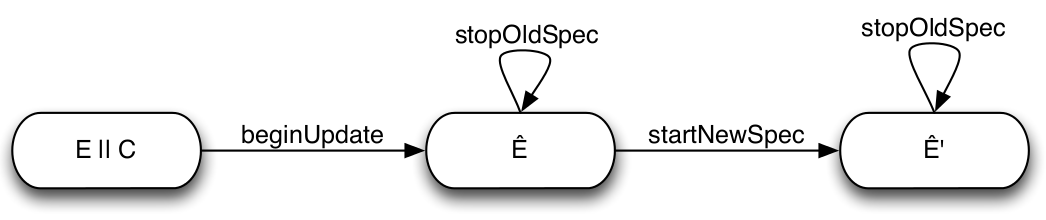
\includegraphics[scale=0.35]{img/E_u.png}
\caption{Representación gráfica del ambiente $E_u$ para el problema de control de la actualización de controladores
dinámicamente - $\hat{E}$ es $E$ con la diferencia de que su estado inicial es el estado actual de $E$ en $E\|C$.
$\hat{E'}$ es $E'$ con la diferencia de que su estado inicial es alguno de los estados relacionados en $M$ con el estado
actual de $E$.}
\label{update_environment}
\end{figure}

Las definiciones anteriores construyen a $E_u$ para comportarse exactamente igual a $E\|C$ (ver reglas 1 y 2) hasta que
sucede $beginUpdate$. La regla 2 simplemente renombra acciones controladas de $C$ para impedir que el controlador de
actualización las controle. Juntas, ambas reglas permiten intercambiar $C$ por $C_u$ mientras aseguramos que $C_u$
continua ejecutando exactamente de la misma manera que $C$. Una vez que $beginUpdate$ se efectua (regla 3), el ambiente
se comporta como $E$ (regla 4). Es justo en este momento que el nuevo controlador tendrá que mantener la vieja
especificación pero forzandolo a llegar a un estado desde el cual los requerimientos de transición puedan ser
satisfechos y luego alcanzar la nueva especificación. En cualquier momento el controlador puede efectuar la acción
$stopOldSpec$ (regla 5) e incluso $startNewSpec$ (regla 7). En caso de que ya haya ocurrido la acción $startNewSpec$, el
ambiente de actualizacion $E_u$ se comporta como el nuevo ambiente $E'$ (regla 8). Aunque como no forzamos que la
vieja especificación deje de valer antes de que valga la nueva especificación, $stopOldSpec$ puede ocurrir durante esta
última fase (regla 6).

\subsection{El problema de control de la actualización de controladores dinámicamente}

Ahora podemos definir formalmente el problema de control que nos soluciona el escenario de la actualización de
controladores dinámicamente.

El problema de control de la actualización de controladores dinámicamente puede ser visto como un problema de control de
LTS usando un ambiente $E_u$ como definimos en la definición \ref{update_environment_def}, los objetivos $G_u$ como
definimos en la definición \ref{update_goals_def} y el conjunto de acciones controlables $A_u$ definido como la unión de las
acciones controlables entre $A$ y $A'$. La única sutileza es que como $E_u$ introduce cambios de nombres de acciones que
son controladas por $C$ en la primera fase ($E\|C$), estos cambios deben ser revertidos una vez computado el controlador
de actualización (reemplazar las acciones $\bar{\ell}$ por $\ell$). Recordar que el cambio de nombre es realizado para
asegurar que el controlador de actualización, cuando se esta generando, no considere a las acciones de $E\|C$ como
controlables hasta que suceda $beginUpdate$. Una vez computado, mientras el controlador de actualización es ejecutado
las acciones deben ser revertidas a su nombre original.

\begin{nahaDef}
\emph{(El problema de control de la actualización de controladores dinámicamente) Sean $G$ y $G'$ expresiones de flujos
sin expresiones temporales. Sea $E$ un LTS y sea la formula FLTL $\Box G$ la especificación actual que el sistema esta
satisfaciendo tras ejecutar el LTS $C$, controlador que controla las acciones en $A$. Sea $E'$ un LTS, la formula FLTL
$\Box G'$ y un conjunto de acciones controlables $A'$ la nueva especificación que es esperada satisfacer con la
actualización dinámica del controlador del sistema.}

\emph{$C_u$ es una solución al problema de control de actualización de controladores dinámicamente si $C_u$ es el resultado de
renombrar toda acción $\bar{\ell}$ por $\ell$ en el controlador $\overline{C}$ que es una solución al problema de
control LTS $\langle E_u, G_u, A_u \rangle$ donde $E_u$ esta definido en la definición \ref{update_environment_def},
$G_u$ esta definido en la definición \ref{update_goals_def} y $A_u = A \cup A'$.}
\end{nahaDef}

\begin{figure}
\centering
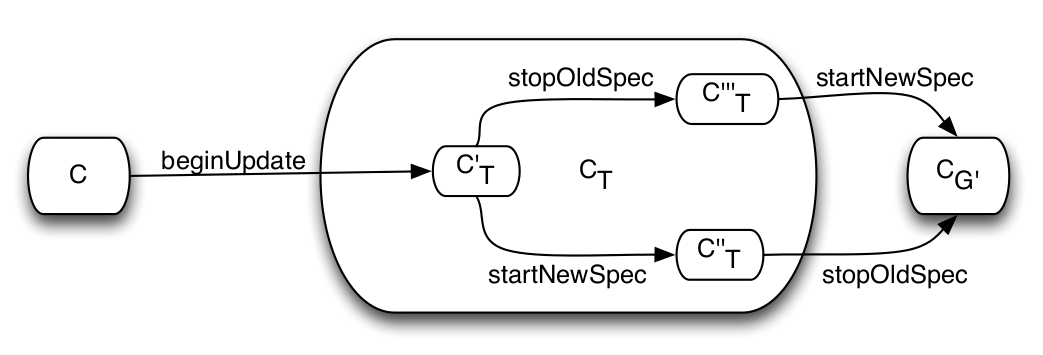
\includegraphics[scale=0.35]{img/C_u.png}
\caption{Abstracción informal de un controlador $C_u$ para el problema de control de la actualización de controladores
dinámicamente - $C_T$ representa el comportamiento que satisface $T$ mientras que garantiza eventualmente tanto
$stopOldSpec$ como $startNewSpec$, mientras que $C_{G'}$ representa el comportamiento del controlador que satisface
$G'$.}
\label{update_controller}
\end{figure}

Por definición, cualquier solución del problema de control de la actualización de controladores dinámicamente
satisfacerá a $G_u$ asumiendo que el ambiente se comporta como $E_u$. La validez de las asunciones de $E_u$ dependen en
la validez de las especificaciones actuales y nuevas, $E$ y $E'$, que son responsabilidad del ingeniero, y que la
infraestructura de ejecución del controlador va a dinámicamente cargar cualquier nueva habilidad descrita en $E'$ cuando
la señal $startNewSpec$ suceda.

Un controlador que es solución del problema definido recientemente tomará, informalmente, la estructura descrita en la
Figura \ref{update_controller}. Primero va a comportarse como $C$ excepto que aceptará en cualquier momento que la acción no controlable
$beginUpdate$ suceda. Luego, se comportará como un controlador que esta intentando realizar las acciones $stopOldSpec$ y
$startNewSpec$ mientras satisface la propiedad $T$. Finalmente, una vez que la acción $startNewSpec$ ha ocurrido se
comportará como un controlador que satisface $G'$.


